\documentclass[final,3p,times,twocolumn]{elsarticle}

%% Use the option review to obtain double line spacing
%% \documentclass[preprint,review,12pt]{elsarticle}

%% Use the options 1p,twocolumn; 3p; 3p,twocolumn; 5p; or 5p,twocolumn
%% for a journal layout:
%% \documentclass[final,1p,times]{elsarticle}
%% \documentclass[final,1p,times,twocolumn]{elsarticle}
%% \documentclass[final,3p,times]{elsarticle}
%% \documentclass[final,3p,times,twocolumn]{elsarticle}
%% \documentclass[final,5p,times]{elsarticle}
%% \documentclass[final,5p,times,twocolumn]{elsarticle}

%% if you use PostScript figures in your article
%% use the graphics package for simple commands
%% \usepackage{graphics}
%% or use the graphicx package for more complicated commands
%% \usepackage{graphicx}
%% or use the epsfig package if you prefer to use the old commands
%% \usepackage{epsfig}

%% The amssymb package provides various useful mathematical symbols
\usepackage{amssymb}
%% The amsthm package provides extended theorem environments
%% \usepackage{amsthm}
%% The bm package lets you access bold symbols in math mode using the \boldsymbol command (useful to get bold greek letters).
\usepackage{bm}
%% The bbm (and also dsfont) package is contains the indicator function symbol \mathbbm{1}
\usepackage{bbm}
\usepackage{dsfont}
%% The amsmath package contains the split environment, letting you split equations into multiple lines.
%% See "https://www.sharelatex.com/learn/Aligning_equations_with_amsmath " for an explanation.
\usepackage{amsmath}
%% The lineno packages adds line numbers. Start line numbering with
%% \begin{linenumbers}, end it with \end{linenumbers}. Or switch it on
%% for the whole article with \linenumbers after \end{frontmatter}.
%% \usepackage{lineno}
%% The algorithm package defines the algorithm floating environment and the algpseudocode package is useful for constructing Pseudo code.
\usepackage{algorithm}
\usepackage{algpseudocode}
%% For making algorithms float
\usepackage{float}
\newfloat{algorithm}{t}{lop}
%% For drawing pictures inside latex
\usepackage{tikz}
%% For setting the 'DRAFT' watermark
%\usepackage{draftwatermark}
%\SetWatermarkText{DRAFT}
%\SetWatermarkScale{1}

%% Declaring \argmin and \argmax operators:
\DeclareMathOperator*{\argmin}{arg\,min}
\DeclareMathOperator*{\argmax}{arg\,max}
%% Declare trace operator \Tr and covariance \Cov:
\DeclareMathOperator*{\Tr}{Tr}
\DeclareMathOperator*{\Cov}{Cov}
%% Declare pdf functions
\DeclareMathOperator*{\Dir}{Dir}
\DeclareMathOperator*{\Cat}{Cat}
%% shorthand for \boldsymbol and \overline
\let\bs\boldsymbol
\let\ol\overline
%% Indicator symbol
\DeclareMathOperator*{\id}{\mathds{1}}
%% natbib.sty is loaded by default. However, natbib options can be
%% provided with \biboptions{...} command. Following options are
%% valid:

%%   round  -  round parentheses are used (default)
%%   square -  square brackets are used   [option]
%%   curly  -  curly braces are used      {option}
%%   angle  -  angle brackets are used    <option>
%%   semicolon  -  multiple citations separated by semi-colon
%%   colon  - same as semicolon, an earlier confusion
%%   comma  -  separated by comma
%%   numbers-  selects numerical citations
%%   super  -  numerical citations as superscripts
%%   sort   -  sorts multiple citations according to order in ref. list
%%   sort&compress   -  like sort, but also compresses numerical citations
%%   compress - compresses without sorting
%%
%% \biboptions{comma,round}

% \biboptions{}


\journal{MPhil in Scientific Computing}

\begin{document}

\begin{frontmatter}

%% Title, authors and addresses

%% use the tnoteref command within \title for footnotes;
%% use the tnotetext command for the associated footnote;
%% use the fnref command within \author or \address for footnotes;
%% use the fntext command for the associated footnote;
%% use the corref command within \author for corresponding author footnotes;
%% use the cortext command for the associated footnote;
%% use the ead command for the email address,
%% and the form \ead[url] for the home page:
%%
%% \title{Title\tnoteref{label1}}
%% \tnotetext[label1]{}
%% \author{Name\corref{cor1}\fnref{label2}}
%% \ead{email address}
%% \ead[url]{home page}
%% \fntext[label2]{}
%% \cortext[cor1]{}
%% \address{Address\fnref{label3}}
%% \fntext[label3]{}

\title{Implementation and Comparison of the $K$-Means algorithm and the Gaussian Mixture Model}

%% use optional labels to link authors explicitly to addresses:
%% \author[label1,label2]{<author name>}
%% \address[label1]{<address>}
%% \address[label2]{<address>}

\author{Brian Azizi}

\address{Cavendish Laboratory, Department of Physics, J J Thomson
  Avenue, Cambridge. CB3 0HE}

\begin{abstract}
With the accelerating amount of unstructed information in the world, unsupervised machine learning gains in importantance.
Clustering is one of the main tools for knowledge discovery within machine learning.
This paper provides a summary of $K$-means clustering and the Gaussian mixture model, two of the most widely used clustering techniques.
We will describe our implementation of the methods and give a detailed derivation of their theoretical foundation.
\end{abstract}

\end{frontmatter}

%%
%% Start line numbering here if you want
%%
% \linenumbers

%% main text
\section{Introduction}
\label{sect:Intro}
The goal of \emph{clustering} (also known as \emph{cluster analysis}) is to divide a set of data points into different clusters such that data points withing the same cluster are similar to each other and dissimilar to data points in different clusters. 
When faced with an unlabeled and high-dimensional data set, performing a cluster analysis can give us a few useful initial insights into the underlying system.

Due its general use as a tool for knowledge discovery, clustering has found practical applications in range of disciplines.
In Biology, and particularly in genetic cluster analysis, clustering methods have been used to infer structures in genetic population.
Clustering has become a common tool in market research, allowing for automatic market segmentation.
More recently, text clustering has been used by Google News to aggregate reports on a particular news story from many different publications.
Another common use of clustering is in methods of automatic image segmentation. Important applications of image segmentation include medical imaging and machine vision.

This paper introduces two of the most widely used approaches to clustering, the $K$-means algorithm and the \emph{Gaussian mixture model}.
We have provided a general discussion and derivation of both methods as well as a description of their implementation.

We begin in section \ref{sect:kmeans} by describing and deriving the standard $K$-means algorithm.
Section \ref{sect:EM} gives an abstract description of mixture models and latent variable models in general.
It also derives the expectation-maximization algorithm which is one of the most important tools in machine learning.
We then give a treatment of Gaussian mixture models in section \ref{sect:gmm}.
Finally, we discuss extensions and conclude in section \ref{sect:concl}.

\section{$K$-Means Clustering}
\label{sect:kmeans}
In this section we introduce the \emph{$K$-Means algorithm} \cite{lloyd1982}.
It is one of the simplest and most intuitive approaches to clustering.
The algorithm requires only a single parameter to be set, namely the number of desired clusters $K$. 
It outputs a \emph{flat} and \emph{non-probabilistic} clustering of the data.

We start off by giving a general description of the method and stating the algorithm.
Following that, we look at its convergence properties and derive the formulas used in the algorithm.
We then discuss model selection in the context of $K$-means clustering and demonstrate the algorithm in a simple setting.
We finish the section with a brief discussion of extensions and generalizations of $K$-means.



\subsection{The $K$-Means algorithm}
Suppose we have data set $S = \{\bs x^{(1)},\dots,\bs x^{(N)}\}$ consisting of $N$ observations of the $D$ dimensional random variable $\bs X \in \mathbb{R}^D$.
We would like to partition the data into $K$ sets, where each set corresponds to a cluster.
For now, we assume that $K$ is given. In section \ref{sect:kmeans-ms}, we will discuss some common strategies for how $K$ can be set.

\begin{algorithm}
\caption{$K$-Means algorithm}
\label{alg:kmeans}
\begin{algorithmic}[1]
\State Initialize cluster centroids $\bs\mu_1,\dots,\bs\mu_K$
\Statex
\Repeat
\For{$i = 1,\dots,N$}
\State $z^{(i)} := \argmin_k ||\bs x^{(i)} - \bs\mu_k||^2$
\EndFor
\Statex
\For{$k = 1,\dots,K$}
\State $\bs\mu_k := \frac{\sum_{i=1}^N \id \{z^{(i)}\,=\,k\}\, \bs x^{(i)}}{\sum_{i=1}^N \id\{z^{(i)}\,=\,k\}}$
\EndFor
\Until{Convergence}
\Statex\State\Return{$z^{(1)}, \dots, z^{(N)}, \bs\mu_1, \dots, \bs\mu_K$}
\end{algorithmic}
\end{algorithm}

Each cluster $k$ is represented be a \emph{cluster centroids} $\bs\mu_k \in \mathbb{R}^D$.
We also need to introduce a latent variable $z^{(i)}$ for each data point $x^{(i)}$ that contains the \emph{cluster assignment} for sample $i$.
If $z^{(i)} = k$, then $x^{(i)}$ belongs to cluster $k$.

The $K$-Means algorithm starts by initializing the centroids $\boldsymbol \mu_k$.
Typically, this is done by randomly selecting $K$ distinct data points as the initial values for the centroid variables.

\begin{figure*}
\centering
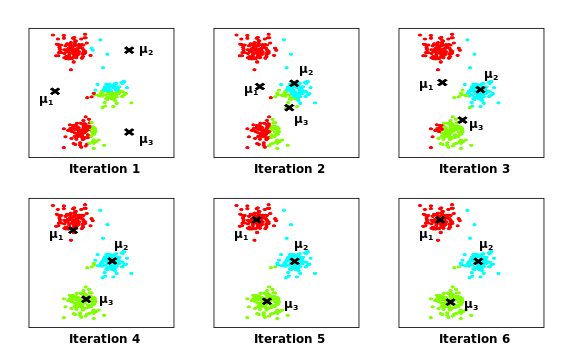
\includegraphics[width=\textwidth,height=3.9in]{prog.png}
\caption{Illustration of the $K$-means algorithm on a 2d data set with $K=3$.
Cluster assignment is shown by colour. The algorithm converges in 6 iterations}
\label{fig:kmeans-prog}
\end{figure*}

The algorithm then repeats the following two steps until convergence:
\begin{enumerate}
\item Assign each sample $x^{(i)}$ to the cluster represented by the centroid $\bs\mu_k$ that is closest to it.
\item Assign each cluster centroid $\bs\mu_k$ to the mean of all samples that currently belong to cluster $k$.
\end{enumerate}
The algorithm has converged once there are no more changes.
We have summarized the $K$-means algorithm in Algorithm \ref{alg:kmeans}.

Figure \ref{fig:kmeans-prog} illustrates the algorithm with $K=3$ on a 2d data set consisting of 300 data points.
We chose a poor initialization for the cluster centroids so that we could show several iterations. 
With a better initialization, as suggested above, convergence would have been faster.



\subsection{Derivation and Convergence of $K$-Means}
\label{sect:kmeans-derivation}
In order to prove convergence of $K$-means, we define the \emph{distortion function} 
\begin{equation}
\label{eqn:distortion}
J(z^{(1)},\dots,z^{(N)},\bs\mu_1,\dots,\bs\mu_K) = \sum_{i=1}^N \sum_{k=1}^K \id\{z^{(i)}=k\}\,||\bs x^{(i)} - \bs \mu_k||^2
\end{equation}
The objective of $K$-Means clustering is equivalent to finding the parameters $z^{(i)} \in \{1,\dots,K\}$ and $\bs\mu_k\in\mathbb{R}^D$, for all $i$ and $k$, that minimize the distortion function $J$.

The $K$-means is obtained by applying the \emph{coordinate descent algorithm} to minimize the distortion function.
Coordinate descent is a simple optimization algorithm that can be used to find a local minimum of a multivariate function $F(\bs y)$.
It starts off by forming an initial guess $\bs y^{0}$ for the minimum $\bs y^*$. 
It then repeatedly cycles through each coordinate direction $y_j$ and minimizes $F$ along that direction.

In the case of the distortion function $J$, we only need to initialize the cluster centroids since the cluster assignments are independent of one another (the optimal value for $z^{(i)}$ tells us nothing about what $z^{(j)}$ should be).
We then minimize $J$ with respect to each $z^{(i)}$ keeping all other variables constant. 
If $K$ and $N$ are not too large, we can do this optimization by individually trying each value for $z^{(i)}$, i.e. by brute force.
The optimal value for $z^{(i)}$ is given by
\begin{equation}
\label{eqn:kmeans-E}
z^{(i)} = \argmin_k ||\bs x^{(i)} - \bs\mu_k||^2
\end{equation}
giving us the first inner loop of the $K$-means algorithm (lines 3-5 in algorithm \ref{alg:kmeans}).

Next, we minimize $J$ with respect to each cluster centroid $\bs\mu_k$ keeping all other variables constant.
We can do so by setting the gradient of $J$ with respect to $\bs\mu_k$ to zero:
\begin{equation}
\label{eqn:kmeans-M0}
\begin{split}
\nabla_{\bs\mu_k} J &= \nabla_{\bs\mu_k} \sum_{i=1}^N\id\{z^{(i)}=k\}(\bs x^{(i)}-\bs\mu_k)^T(\bs x^{(i)}-\bs\mu_k)\\
&= -2 \sum_{i=1}^N\id\{z^{(i)}=k\}(\bs x^{(i)}-\bs\mu_k) = 0\\
\end{split}
\end{equation}
Rearranging this equation gives us
\begin{equation}
\label{eqn:kmeans-M}
\Rightarrow \bs\mu_k = \frac{\sum_{i=1}^N\id\{z^{(i)} = k\}\,\bs x^{(i)}}{\sum_{i=1}^N\id\{z^{(i)}=k}
\end{equation}
This is the second inner loop of the algorithm (lines 6-8 in algorithm \ref{alg:kmeans}).
Furthermore, as already mentioned, (\ref{eqn:kmeans-M}) corresponds to setting $\bs \mu_k$ to the means of all samples $\bs x^{(i)}$ which currently assigned to cluster $k$.
\footnote{It is possible that $\sum_{i=1}^N\id\{z^{(i)}=k\} = 0$.
In other words, there is a possibility that a cluster becomes empty in the course of the algorithm.
If this happens, we can simply re-initialize the corresponding cluster centroid.
However, this may be an indication that we have set $K$ too large.}

One property of the coordinate descent algorithm is that each iteration is a (weak) improvement on the previous one.
This can be easily seen by noting that no update can make us worse off. 
So if the approximation to the solution at iteration $j$ is $\bs y^{(j)}$, then $F(\bs y^{(j)}) \geq F(\bs y^{(j+1)})$.
Hence, as long as the objective function is bounded below, the algorithm is guaranteed to converge to a local minimum.
Using the fact that $J \geq 0$, we have thus established convergence of the $K$-means algorithm.

Note, however, that we are only guaranteed to converge to a \emph{local} minimum.
Figure \ref{fog:kmeans-local} shows an example of a local optimum of the $K$-means algorithm applied to the same data set as in Figure \ref{fig:kmeans-prog}.

In two dimensions, we are able to visualize the data and might be able to identify a local solution simply by looking at the outcome. 
This is more difficult to do in higher dimensions.
In practice, this problem is dealt with by performing multiple runs of the entire $K$-Means algorithm.
We have to make sure that each run uses a different set of initial values for the the cluster centroids since, given an initialization, the $K$-means algorithm is completely deterministic.
We also need to record the final value of the distortion function $J$ after each run.
The overall output is then chosen to be the solution corresponding to the run for which the final value of $J$ was smallest.
Although this method does not guarantee convergence to the global optimum either, the resulting outcome is usually accepted to be at least ``good enough".

Convergence of the $K$-means algorithm was extensively studied by \cite{macqueen1967}.

\begin{figure}
\centering
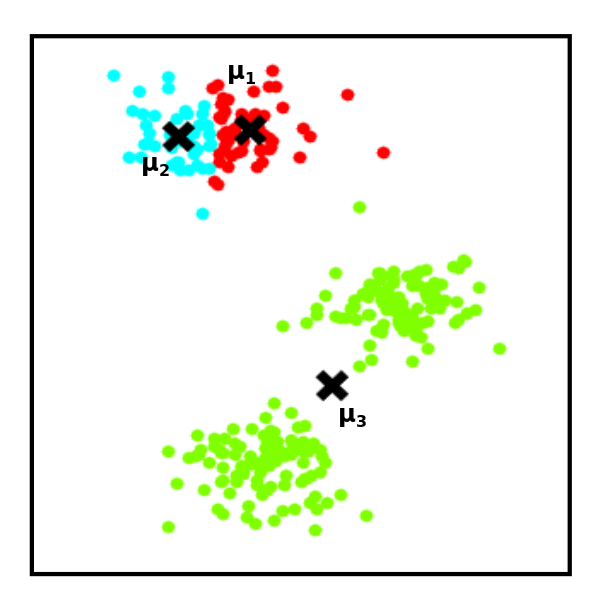
\includegraphics[width=3in]{local.png}
\caption{Local optimum of the K-Means algorithm applied to the data set from Figure \ref{fig:kmeans-prog} with $K=3$.}
\label{fig:kmeans-local}
\end{figure}


\subsection{Model selection for $K$-Means Clustering}
\label{sect:kmeans-ms}

\begin{figure*}
\centering
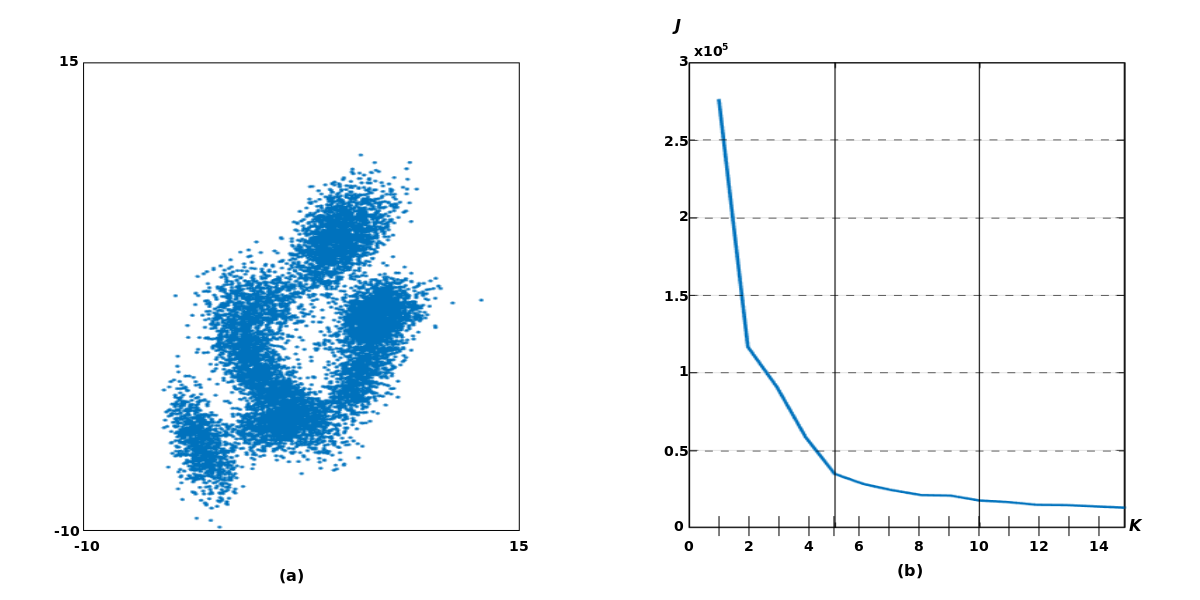
\includegraphics[width=\textwidth,height=3in]{elbow.png}
\caption{Illustration of the elbow method for selecting $K$ in $K$-means clustering. 
(a) Example 2d data set.
(b) We ran $K$-means on the data set in (a) for $1\leq K\leq 15$ and plotted the optimal value of the distortion function $J$ against $K$.}
\label{fig:kmeans-elbow}
\end{figure*}

The only user-set parameter in the $K$-means algorithm is the number of clusters.
Therefore, model selection for $K$-means amounts to selecting the optimal value for $K$.

The standard model selection tool for $K$-means clustering is the so-called ``elbow method" (also referred to as the ``kink method").
We run the $K$-Means algorithm for a range of different values of $K$, say for $1 \leq K \leq K_{max}$, where $K_{max}$ is some preset maximum value for $K$.
For each run, the optimal value of the distortion function, $J^*_K$, is saved.
If necessary, perform multiple random initializations for each $K$ to avoid poor local optima.
Finally, we plot $J_K^*$ against $K$.

In some cases, it is possible to identify a distinct ``kink" in the curve at some $K^*$ (i.e. the curve has a noticable ``elbow").
If that is the case, it would be a reasonable choice to set $K$ to the value at which the kink occurs.

The intuition is that, if there is some true number of clusters $K^*$, we would expect a steep slope in the elbow curve for $K < K^*$.
If $K < K^*$, we are putting several clusters into the same group. 
Splitting the group into its constituent clusters should have a large effect on the distortion function.

If $K > K^*$, we have broken individual clusters into smaller groups.
Thus, we would expect only a small reduction in the distortion compared to $K^*$.

We have illustrated the elbow method in Figure \ref{fig:kmeans-elbow}.
Note the disctinct ``kinks" at $K=3$ and $K=5$.
Looking at panel (a), either choice for $K$ could be a reasonable choice.

In practical applications, the optimal value for $K$ is often ambiguous.
In fact, a common behaviour of real-world data is that the number of clusters grows with the size of the data set.

Because of this, $K$ is usually chosen manually in practice.
In some applications, domain-specific knowledge may provide a reasonable value for $K$.



\subsection{Implementation Details and Demonstration}
\label{sect:kmeans-code}
We have implemented the $K$-means algorithm in C++ using the external linear algebra library ``Armadillo" \cite{armadillo}.
Translating the pseudo-code in algorithm \ref{alg:kmeans} into C++ is straight-forward.
We only added two further features.
\begin{enumerate}
\item We put set a maximum value for the number of iterations in order to put a bound on the running time.
This is not strictly necessary since, as we saw in section \ref{sect:kmeans-derivation}, the algorithm is guaranteed to converge.
\item We run the algorithm multiple times, randomly re-initializing the centroids before each run.
We then save the output of the run for which $J$ was smallest.
As explained in section \ref{sect:kmeans-derivation}, this is done in order to mitigate the risk of getting a poor local optimum.
\end{enumerate}

Possible demo for $K$-means:
\begin{itemize}
\item Image compression
\item MNIST data
\end{itemize}


\label{sect:kmeans-concl}
In the introduction, we said that we would like data points inside the same cluster to be similar to each other and dissimilar to data points in other clusters.

The notion of similarity that we have been using in our discussion so far is based on squared Euclidean distance:
Two points $\bs x$ and $\bs x'$ are dissimilar if $||\bs x-\bs x'||^2$ is large.

It is possible to formulate the $K$-means algorithm using a general dissimilarity metric $V(\boldsymbol x, \boldsymbol x')$.
In that case, the distortion function takes the form
\begin{equation}
\label{eqn:kmedoid-distortion}
J(z^{(1)},\dots,z^{(N)},\bs \mu_1,\dots,\bs \mu_K) = \sum_{i=1}^N \sum_{k=1}^K \id\{z^{(i)}=k\}\,V(\bs x^{(i)}, \bs \mu_k)
\end{equation}
and the resulting algorithm is a generalization of $K$-means known as the \emph{$K$-medoids algorithm}.

Updating the cluster centroids in the $K$-medoids algorithm could be more complicated than in the $K$-means algorithm since the metric $V$ may not offer the same analytical convenience as the squared Euclidean metric.
One possible way of dealing with this problem is to restrict the cluster centroids $\bs\mu_k$ to be one of the data points $\bs x^{(i)}$ in cluster $k$.
This can be implemented as discrete search over the cluster.

Further extensions of the $K$-means algorithm are achieved by improving the cluster assignment step.
In its current form, we need to compute the squared Euclidean distance a total of $K$ times for each of the $N$ data points.
There have been proposals for speeding up this step (see \cite{Bishop} for a discussion and references).

In section \ref{sect:gmm}, we will discuss the Gaussian mixture model which can be regarded as a generalization of $K$-means to a probabilistic framework.

For more information on K-Means clustering, consult \cite{Bishop,Murphy}.






\section{Mixture Models and the EM Algorithm}
\label{sect:fmm}
The $K$-means algorithm provided us with a \emph{hard clustering} of the data.
This means that every data point $\bs x^{(i)}$ was assigned to a single cluster and we have no way of measuring the confidence of that assignment.
It could be that $\bs x^{(i)}$ ends up being very close to its cluster's centroid in which case the hard assignment is reasonable.
But it may also happen that $\bs x^{(i)}$ ends up being roughly midway between two centroids.
In that case, the hard assignment to the nearest centroid seems a lot less appropriate.

Ideally, we would like our cluster assignments to come with a measure of confidence, a so-called \emph{soft clustering}.
This section introduces a popular and simple approach to soft clustering.
We estimate the density of the data using a mixture model with $K$ components.
This will provide us with a posterior probabilities of each sample $\bs x^{(i)}$ belonging to the individual components of the model.
By viewing the components of the model, we end up with a soft clustering of our data into $K$ clusters.

We start off with a general desciption of finite mixture models in section \ref{sect:mixtures}.
We then discuss how to fit the parameters of the model using the \emph{EM algorithm}.

This section introduces mixture models and the EM algorithm in a general framework.
In section \label{sect:gmm}, we will discuss Gaussian mixtures, the most popular instance of finite mixture models.





\subsection{Mixture Models}
\label{sect:mixtures}
Suppose we have a data set $S = \{\bs x^{(1)},\dots,\bs x^{(N)}\}$ consisting of $N$ independent observations of a random variable $\bs X \in \mathbb{R}^D$.
We are interested in modelling the distribution of $\bs X$, i.e. we would like to use the data $S$ to estimate the probability density function $p(\bs x)$ of $\bs X$.

There are many ways of tackling this problem. 
The standard approach is to assume that $p(\bs x) = f(\bs x|\,\theta)$, i.e. that $p(\bs x)$ belongs to some family of distributions parametrized by $\theta$ and then use the data set $S$ to estimate $\theta$ with some inference method.
For example, a common technique is to assume $X$ is a Gaussian variable, such that 
\begin{equation}
f(\bs x |\,\theta) = \mathcal{N}(\bs x|\,\bs\mu,\bs \Sigma)
\end{equation}
and then use maximum likelihood estimation to infer the value of the parameter $\theta = (\bs\mu,\bs\Sigma)$.

The standard approach works well for simple data sets, but is somewhat limitted in more complex systems.
A simple way of extending this method is to assume that $p(\bs x)$ is composed of $K$ \emph{base distribution}.
Let $f_k(\bs x)$ denote the density function of the $k$th base distribution $F_K$.
The resulting density of $\bs X$ is then
\begin{equation}
\label{eqn:mixtures}
p(\bs x) = \sum_{k=1}^K \pi_k f_k(\bs x)
\end{equation}
We require $pi_k \geq 0$ for all $k$ and $\sum_{k=1}^K = 1$ in order for the density function to be well-defined.
Models of the form (\ref{eqn:mixtures}) are called \emph{mixture models}.

Mixture models are a special case of \emph{latent variable models}.
To see why, suppose we have discrete latent variable $Z$ taking values in $\{1,\dots,K\}$.
The distribution of $Z$ is fully specified by the quantities $\pi_1,dots,\pi_K$, where $\pi_k = \Pr(Z = k)$, and is referred to as the \emph{categorical distribution}, denoted $Z \sim \Cat(\pi_1, \dots,\pi_K)$.
We can express the probability mass function of $Z$ by
\begin{equation}
\label{eqn:cat}
\Cat(z|\,\bs\pi) = \prod_{k=1}^K \pi_k^{\id\{z=k\}}
\end{equation}
Note that, due their probabilistic nature, the parameters $\bs \pi = (\pi_1,\dots,\pi_K)$ must satisfy $\pi_k \geq 0$, $\sum_{k=1}^K \pi_k = 1$.

Our mixture models can then be built as follows:
\begin{equation}
\begin{split}
\label{eqn:mixture-lvm}
Z &\sim \Cat(\bs\pi)\\
\bs X |\,Z=k &\sim F_k
\end{split}
\end{equation}
The joint distribution of $\bs X$ and $Z$ is obtained from the product rule of probability:
\begin{equation}
\label{eqn:product-rule}
p(\bs x, z) = p(z)p(\bs x|\,z)
\end{equation}
Finally, to get the marginal ditribution of $\bs X$, we apply the sum rule of probability:
\begin{equation}
\label{eqn:sum-rule}
p(\bs x) = \sum_z p(\bs x, z)
\end{equation}

The resulting model is then derived as follows
\begin{equation}
\label{eqn:mixture-derivation}
\begin{split}
p(\bs x) &= \sum_z p(\bs x, z)\\
&= \sum_z p(z)p(\bs x|\,z)\\
&= \sum_{k=1}^K \Pr(Z=k) p(\bs x|\,Z=k)\\
&= \sum_{k=1}^K \pi_k f_k(\bs x)
\end{split}
\end{equation}
This is the same as the mixture model in (\ref{eqn:mixtures}).

Typically, the base distributions are chosen to belong to the same parametric family and differ only in the value of their parameter, so that $f_k(\bs x) = f(\bs x|\, \theta_k)$.
In that case, the mixture distribution is given by
\begin{equation}
\label{eqn:mixture-model}
p(\bs x|\,\bs\pi,\bs\theta) = \sum_{k=1}^K \pi_k f(\bs x|\,\theta_k)
\end{equation}
where we have made the dependence on the parameters $\bs\pi$ and $\bs\theta = (\theta_1,\dots,\theta_K)$ explicit.


\subsection{The EM algorithm}
\label{sect:EM}
Given our data set $S=\{\bs x^{(1)},\dots,\bs x^{(N)}\}$, how do we infer the parameters of our mixture model (\ref{eqn:mixture-model})?
The standard inference method in frequentist statistics is to find the parameter value that maximizes the likelihood of the data. 
So if our model for the joint distribution of $\bs X$ is $p(\bs x|\,\bs\theta)$, the likelihood of our data set $S$ is given by
\begin{equation}
\label{eqn:likelihood}
\mathcal{L}(\bs\theta) = \prod_{i=1}^N p(\bs x^{(i)}|\,\bs \theta)
\end{equation}
and we would like to find $\bs \theta$ that maximises $\mathcal{L}(\bs\theta)$.
This inference method is known as \emph{maximum likelihood estimation}. 

For simple models this problem can often be solved analytically.
Unfortunately, this is generally not the case for latent variable models and mixture models, in particular.

In this section, we will introduce the \emph{Expectation-Maximization} (EM) algorithm \cite{dempster1977}.
It is powerful variational technique that can be used to find a maximum likelihood solution in models with latent variables.

In a general latent variable framework, we have a model for $p(\bs x,z\,|\,\bs\theta)$, the joint distribution of the observed variable $\bs X$ and the latent variable $Z$ with parameter $\bs\theta$. 
The log likelihood of the data $S$ is 
\begin{equation}
\label{eqn:EMlikelihood}
\begin{split}
\ell(\bs\theta) &= \sum_{i=1}^N \log p(\bs x^{(i)}|\,\bs\theta)\\
&= \sum_{i=1}^N \log \left( \sum_{z^{(i)}} p(\bs x^{(i)},z^{(i)}|\,\bs\theta)\right)
\end{split}
\end{equation}
The sum inside the logarithm is what generally makes this optimization problem analytically intractable.
The expectation-maximization algorithm uses a simple iterative approach, often with closed-form updates at each step.
It alternated between two steps.
In the expectation (E) step, it forms a function that is a lower bound to $\ell(\bs\theta)$ and that is tight at the current value of $\bs\theta$.
In the maximization (M) step, it finds $\bs\theta$ that maximizes this lower bound.
This guarantees that we increase the value of $l(\theta)$ in each step until we find a local maximum.

In the following, we will derive the general form of the EM algorithm for maximizing the log likelihood function (\ref{eqn:EMlikelihood}).
We are treating $Z$ as a discrete latent variable, but the derivation is analogous for continuous $Z$ by simply exchanging the relevant sums with integrals.

We start by letting $Q_i(z^{(i)})$ be any probability function for $Z^{(i)}$. 
That means $Q_i(z^{(i)}) \geq 0$ and $\sum_{z^{(i)}} Q_i(z^{(i)}) = 1$. 
Our objective function can then be expressed as
\begin{equation}
\begin{split}
\ell(\bs\theta) &= \sum_{i=1}^N \log\left(\sum_{z^{(i)}} p(\bs x^{(i)},z^{(i)}\,|\,\bs\theta)\right)\\
&= \sum_{i=1}^N \log \left(\sum_{z^{(i)}} Q_i(z^{(i)}) \frac{p(\bs x^{(i)},z^{(i)}\,|\,\bs\theta)}{Q_i(z^{(i)})}\right)\\
&= \sum_{i=1}^N \log \mathbb{E}_{z^{(i)} \sim Q_i}\left[\frac{p(\bs x^{(i)},z^{(i)}\,|\,\bs\theta)}{Q_i(z^{(i)})}\right]\\
\end{split}
\end{equation}
where we used the definition of the expectation operator.

\begin{figure}
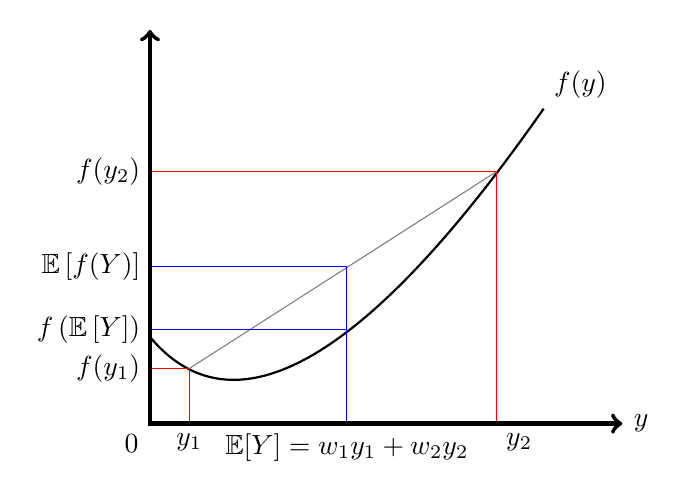
\begin{tikzpicture}
\draw [thick] (0,1.1) [out=310,in=235] to (5,4) node [above right] {$f(y)$};
\draw [gray] (0.5,0.7) -- (4.4,3.2);
\draw [thin, red] (0.5,0.7) -- (0.5,0) node [black,below] {$y_1$};
\draw [thin, red] (4.4,3.2) -- (4.4,0) node [black,below right] {$y_2$};
\draw [thin, red] (0.5,0.7) -- (0,0.7) node [black,left] {$f(y_1)$};
\draw [thin, red] (4.4,3.2) -- (0,3.2) node [black, left] {$f(y_2)$};
\draw [thin, blue] (2.5,2) -- (2.5,0) node [black, below] {$\mathbb{E}[Y]=w_1y_1+w_2y_2$};
\draw [thin, blue] (2.5,2) -- (0,2) node [black, left] {$\mathbb{E}\left[f(Y)\right]$};
\draw [thin, blue] (2.5,1.2) -- (0,1.2) node [black, left] {$f\left(\mathbb{E}\,[Y]\right)$};
\draw [ultra thick,<->] (0,5) -- (0,0) [below left] node{$0$} -- (6,0) node [right] {$y$};
\end{tikzpicture}
\caption{Illustration of Jensen's Inequality.
The random variable $Y$ can take two possible states $y_1$ and $y_2$ with probabilities $w_1$ and $w_2=1-w_1$ respectively.
It $Y$ had only one possible state, say $y_1$, so that $\Pr(Y=y_1)=1$, then $f\left(\mathbb{E}[Y]\right)$ and $\mathbb{E}\left[f(Y)\right]$ would coincide.
}
\label{fig:jensen}
\end{figure}

To proceed, we make use of \emph{Jensen's Inequality}:
Let $Y$ be a random variable and $f$ a convex function. Then
\begin{equation}
f\left(\mathbb{E}[Y]\right) \leq \mathbb{E}\left[f(Y)\right]
\label{eqn:jensen}
\end{equation}
Further, if $f$ is strictly convex, then the inequality is strict and we have
\begin{equation}
\mathbb{E}\left[f(Y)\right] = f\left(\mathbb{E}[Y]\right) \iff \Pr\left(Y = E[Y]\right) = 1
\label{eqn:jensentight}
\end{equation}
An illustration of Jensen's inequality is shown in Figure \ref{fig:jensen}.
If $f$ is concave, then the holds in inequality reverse since $(-f)$ is convex in that case. 

\begin{algorithm}
\caption{The EM algorithm for LVMs}
\label{alg:EM}
\begin{algorithmic}[1]
\State Initialize $\bs\theta^{\,(current)}$
\Statex\Repeat
\Statex \quad\, E-Step:
\For{$i = 1,\dots,N$}
\State $Q_i(z^{(i)}) = p(z^{(i)}\,|\,\bs x^{(i)},\bs\theta^{\,(current)})$
\EndFor
\Statex\Statex \quad\, M-Step:
\State $\bs\theta^{\,(new)} = \argmax_{\bs\theta}\sum_{i=1}^N \sum_{z^{(i)}} Q_i(z^{(i)}) \log \left( \frac{p(\bs x^{(i)},z^{(i)}\,|\,\bs\theta)}{Q_i(z^{(i)})}\right)$
\State Set $\theta^{\,(current)} = \theta^{\,(new)}$
\Until{Convergence}
\Statex\State\Return{  $\bs\theta^{\,(current)},z^{(1)}, \dots, z^{(N)}$}
\end{algorithmic}
\end{algorithm}

Applying Jensen's inequality to (\ref{eqn:EMlikelihood}) and using the fact that the log function is strictly concave gives us
\begin{equation}
\begin{split}
\ell(\bs\theta) &=  \sum_{i=1}^N \log \mathbb{E}_{z^{(i)} \sim Q_i}\left[\frac{p(\bs x^{(i)},z^{(i)}\,|\,\bs\theta)}{Q_i(z^{(i)})}\right]\\
&\geq \sum_{i=1}^N \mathbb{E}_{z^{(i)} \sim Q_i}\left[\log \frac{p(\bs x^{(i)},z^{(i)}\,|\,\bs\theta)}{Q_i(z^{(i)})}\right]\\ 
&= \sum_{i=1}^N \sum_{z^{(i)}} Q_i(z^{(i)}) \log \left(\frac{p(\bs x^{(i)},z^{(i)}\,|\,\bs\theta)}{Q_i(z^{(i)})}\right) := J(\bs\theta,\bs Q)
\end{split}
\end{equation}
where we used $\bs Q$ to denote $\{Q_1,\dots,Q_N\}$.

$J(\bs\theta,\bs Q)$ is a lower bound to the log likelihood function $\ell(\bs\theta)$ for \emph{any} valid choice of probability functions $\bs Q$.
What should our choice for the $Q_i$ be?



\begin{figure}
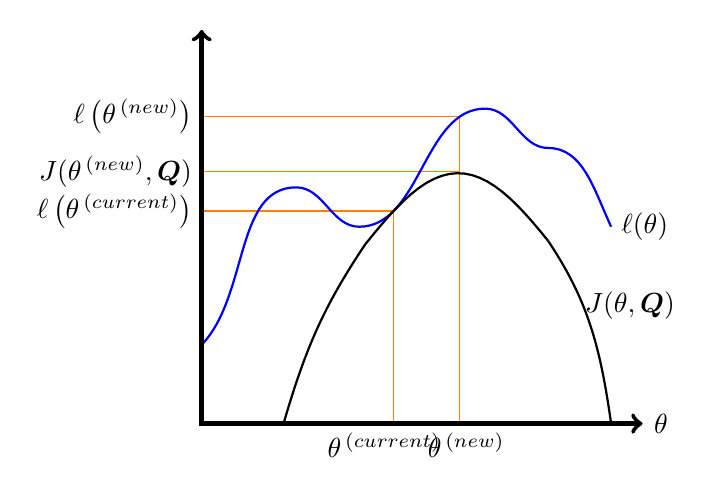
\begin{tikzpicture}[xscale=0.8]
\draw [orange, thin] (3.05,0) -- (3.05,2.7) -- (0,2.7) node [black,left] {$\ell\left(\theta^{\,(current)}\right)$};
\draw [orange, thin] (4.1,0) -- (4.1,3.9) -- (0,3.9) node [black, left] {$\ell\left(\theta^{\,(new)}\right)$};
\draw [orange, thin] (4.1,3.2) -- (0,3.2) node [black,left] {$J(\theta^{\,(new)},\bs Q)$};
\node at (4.2,0) [black, below] {$\theta^{\,(new)}$};
\node at (2.9,0) [black, below] {$\theta^{\,(current)}$};
\node at (6.8,1.5) {$J(\theta,\bs Q)$};
\draw [blue,thick] (0,1) [out=40,in=180] to (1.5,3);
\draw [blue,thick] (1.5,3) [out=0,in=180] to (2.5,2.5);
\draw [blue,thick] (2.5,2.5) [out=0,in=180] to (4.5,4);
\draw [blue,thick] (4.5,4) [out=0,in=180] to (5.5,3.5);
\draw [blue,thick] (5.5,3.5) [out=0,in=120] to (6.5,2.5) node [black,right] {$\ell(\theta)$};
\draw [thick,domain=2.6:5.5] plot (\x, {2.18+(sin((\x - 2.5) r)});
\draw [thick] (1.3,0) [out=70,in=230] to (2.6,2.28);
\draw [thick] (5.5,2.32) to [out=310,in=100] (6.5,0);
\draw [ultra thick,<->] (0,5) -- (0,0) -- (7,0) node [right] {$\theta$};
\end{tikzpicture}
\caption{Illustration of the EM algorithm.
$J(\theta,\bs Q)$ (black curve) is a lower bound to $\ell(\theta)$ (blue curve).
The E-step sets $\bs Q$ such that the blue curve and the black curve touch at $\theta^{\,(current)}$.
The M-step finds $\theta^{\,(new)}$ that maximizes the black curve.
Note how this brings us closer to a maximum of $\ell(\theta)$.}
\label{fig:EM}
\end{figure}

The EM algorithm makes the following choice.
Suppose we currently have an estimate of our parameters $\bs\theta^{\,(current)}$. 
In the E-step, the EM algorithm chooses $Q_i$ so that the lower bound is tight at $\bs\theta^{\,(current)}$, i.e. so that
\begin{equation}
J\left(\bs\theta^{\,(current)},\bs Q\right) = \ell\left(\bs\theta^{\,(current)}\right)
\end{equation}
Jensen's inequality tells us that this can be achieved by setting 
\begin{equation}
\frac{p(\bs x^{(i)},z^{(i)}\,|\,\bs \theta^{\,(current)})}{Q_i(z^{(i)})} = constant
\end{equation}
for all values of $z^{(i)}$.
This implies that
\begin{equation}
Q_i(z^{(i)}) \propto p(\bs x^{(i)},z^{(i)}\,|\,\bs\theta^{\,(current)})
\end{equation}
The constant of proportionality can be calculated by using the constraint that $\sum_{z^{(i)}} Q_i(z^{(i)}) = 1$.
Thus,
\begin{equation}
\label{eqn:EM-E}
\begin{split}
Q_i(z^{(i)}) &= \frac{p(\bs x^{(i)},z^{(i)}\,|\,\bs\theta^{\,(current)})}{\sum_{z^{(i)}}p(\bs x^{(i)},z^{(i)}\,|\,\bs\theta^{\,(current)})}\\
&= \frac{p(\bs x^{(i)},z^{(i)}\,|\,\bs\theta^{\,(current)})}{p(\bs x^{(i)}\,|\,\bs\theta^{\,(current)})}\\
&= p(z^{(i)}\,|\,\bs x^{(i)},\bs\theta^{\,(current)})
\end{split}
\end{equation}
where the second line follows from the sum rule of probability (\ref{eqn:sum-rule}) and the third line follows from the definition of conditional probabilities.

Small digression: These quantities have an important interpretation in the context of soft clustering using mixture models.
They are the posterior distributions of the cluster assignments of our data are referred to as \emph{responsibilities}.
We say that $\Pr(z^{(i)} = k\,|\,\bs x^{(i)},\bs\theta)$ is the responsibility that cluster $k$ takes in explaining sample $\bs x^{(i)}$, and denote it $\gamma_k^{(i)}$.

Setting $Q_i(z^{(i)})$ completes the E-step of the EM algorithm.
In the M-Step, we update our parameters by finding $\bs\theta^{\,(new)}$ that maximizes this lower bound, keeping the $Q_i$ fixed.
In other words, we solve the following optimization problem
\begin{equation}
\label{eqn:EM-M}
\begin{split}
\bs\theta^{\,(new)} &= \argmax_{\bs\theta} J(\bs\theta,\ol{\bs Q}) \\
&= \argmax_{\bs\theta}\sum_{i=1}^N \sum_{z^{(i)}} \ol{Q_i}(z^{(i)}) \log \left( \frac{p(\bs x^{(i)},z^{(i)}\,|\,\bs\theta)}{\ol{Q_i}(z^{(i)})}\right) 
\end{split}
\end{equation}
where $\ol{Q_i}(z^{(i)}) = p(z^{(i)}\,|\,\bs x^{(i)},\bs\theta^{\,(current)})$.
\footnote{Thus, it is possible to interpret the EM algorithm as a particular instance of the coordinate ascent algorithm applied to the function $J(\bs\theta,\bs Q)$.}
This optimization problem is simpler than the direct optimization of the original log likelihood (\ref{eqn:EMlikelihood}).
In particular, it is possible to find a simple closed-form solution for a wide range of models, including the Gaussian mixture model.

We have summarized the general form of the EM algorithm in Algorithm \ref{alg:EM} and Figure \ref{fig:EM} provides an illustration.
An important caveat is that the EM algorithm does not guarantee convergence to the global optimum.
Thus, different initializations of $\bs\theta$ may lead to different outcomes.
However, any particular initialization will always result in the same local optimum.

Thus, similar to the local optima problem in $K$-means, we can try running the EM algorithm multiple times with different initial values in order to increase the chance of obtainint a sufficiently good local optimum.
This is no coincidence as we will see later that the $K$-means algorithm is in fact just an instance of the EM algorithm.

\section{The Gaussian Mixture Model}
\label{sect:gmm}
This section discusses \emph{Gaussian mixture models} (GMM) and their use in clustering.
We begin with a general description of the model.
Next we show how to fit the parameters of the model using the EM algorithm and derive the update formulas.
We then briefly discuss model selection for GMMs.
Following that, we give a short description and demonstration of our implementation of the model before considering possible extensions.

\subsection{Clustering with the Gaussian Mixture Model}
Consider again the general mixture model (\ref{eqn:mixture-lvm}) and the resulting mixture distribution (\ref{eqn:mixture-model}).
The Gaussian mixture model is a particular instance of this model corresponding to the choice $F_k = \mathcal{N}(\bs\mu_k,\bs\Sigma_k)$.
In other words, the GMM is a mixture model with Gaussian base distributions.

The probability density function for a general $D$-dimensional Gaussian variable $\bs X$ is given by
\begin{equation}
\label{eqn:gauss-pdf}
\mathcal{N}(\bs x|\,\bs\mu,\bs\Sigma) = (2\pi)^{-\frac{D}{2}}|\bs\Sigma|^{-\frac{1}{2}}\exp\left((\bs x - \bs\mu)^T\bs\Sigma^{-1}(\bs x-\bs\mu)\right)
\end{equation}
where $\bs\mu = \mathbb{E}[\bs X]$ is the mean parameter and $\Sigma = \Cov(\bs X)$ is the covariance parameter.
The covariance parameter $\bs\Sigma$ is a $D\times D$ symmetric and positive definite matrix, while $\bs\mu$ is a $D$-dimensional vector.

We can express the GMM with $K$ mixture components as
\begin{equation}
\label{eqn:gmm-lvm}
\begin{split}
Z\,|\,\pi_1,\dots,\pi_K &\sim \Cat(\pi_1,\dots,\pi_K)\\
\bs X \,|\,Z=k,\bs\mu_k,\bs\Sigma_k &\sim \mathcal{N}(\bs\mu_k,\bs\Sigma_k)
\end{split}
\end{equation}
and the resulting model for the joint distribution of $\bs X$ is 
\begin{equation}
\label{eqn:gmm-density}
p(\bs x|\,\bs\pi,\bs\mu,\bs\Sigma) = \sum_{k=1}^K \mathcal{N}(\bs x|\,\bs\mu_k,\bs\Sigma_k)
\end{equation}
where we used $\bs\pi$, $\bs\mu$ and $\bs\Sigma$ to denote the collections $(\pi_1,\dots,\pi_K)$, $(\bs\mu_1,\dots,\bs\mu_K)$ and $(\bs\Sigma_1,\dots,\bs\Sigma_K)$, respectively.

How can we used this model to obtain a clustering of a data set $S = \{\bs x^{(1)},\dots,\bs x^{(N)}\}$?
In the model, for each observation $\bs x^{(i)}$, there exists a categorical latent variable $z^{(i)}$ that contains the cluster assignment for $\bs x^{(i)}$.
We do not actually observe $z^{(i)}$ but the model allows us to build their posterior distributions $p(z^{(i)}|\,\bs x^{(i)},\bs \theta)$.
These can be used to specify a soft clustering of the data:
\begin{equation}
\Pr(\mbox{$\bs x^{(i)}$ is in cluster $K$}) = \Pr(z^{(i)} = k|\,\bs x^{(i)},\bs\theta)
\end{equation}
As we mentioned in the previous section, we refer to these quantities responsibilities and denote them with $\gamma_k^{(i)}$.


\subsection{The EM algorithm for the GMM}
The most popular inference method for the GMM is maximum likelihood estimation using the EM algorithm.
Using (\ref{eqn:gmm-density}), we can express the log likelihood of our data set $S$ under the model as
\begin{equation}
\label{eqn:gmmlogLikelihood}
\begin{split}
\ell(\bs\pi,\bs\mu,\bs\Sigma) &= \sum_{i=1}^N \log \left(p(\bs x^{(i)}|\,\bs\pi,\bs\mu,\bs\Sigma\right)\\
&= \sum_{i=1}^N \log \left(\sum_{k=1}^K \pi_k \mathcal{N}(\bs x^{(i)}|\,\bs\mu_k,\bs\Sigma_k)\right)
\end{split}
\end{equation}
Direct maximization of this log likelihood function is analytically intractable and we apply the EM algorithm instead.

We start by setting some initial value for the parameters $\bs\pi^{\,(current)}$, $\bs\mu^{\,(current)}$ and $\bs\Sigma^{\,(current)}$.
This is typically done randomly.
However, we have to be careful when initializing the mixing coefficients $\bs\pi$ since they need satisfy the constraints that $\sum_{k=1}^K \pi_k = 1$ and $\pi_k \geq 0$ for all $k$.
Once an initial value for the parameters is set, the EM algorithm alternates between the E-step and the M-step until some convergence criterion is met.

In the E-step (\ref{eqn:EM-E}), we need to find the $Q_i(z^{(i)})$
In the case of the GMM, this translates to calculating the responsibilities $\gamma_k^{(i)}$ for all values of $i$ and $k$.
Using Bayes' rule, we can derive a simple formula in terms of the current values of the parameter $\bs\pi$, $\bs\mu$ and $\bs\Sigma$:
\begin{equation}
\label{eqn:gmmresponsibility}
\begin{split}
\gamma_k^{(i)} &= \Pr(z^{(i)}=k|\,\bs x^{(i)},\bs\pi,\bs\mu,\bs\Sigma)\\
&= \frac{\Pr(z^{(i)}=k|\,\bs\pi)p(\bs x^{(i)}|\,z^{(i)}=k,\bs\mu,\bs\Sigma)}{\sum_{j=1}^K \Pr(z^{(i)}=j|\,\bs\pi)p(\bs x^{(i)}|\,z^{(i)}=j,\bs\mu,\bs\Sigma)}\\
&= \frac{\pi_k\mathcal{N}(\bs x^{(i)}|\,\bs\mu_k,\bs\Sigma_k)}{\sum_{j=1}^K \pi_j\mathcal{N}(\bs x^{(i)}|\,\bs\mu_j,\bs\Sigma_j)}
\end{split}
\end{equation}
where, for convenience, we have temporarily dropped the ``$(current)$" superscript.

In the M-Step (\ref{eqn:EM-M}), we find the parameters $\bs\pi$, $\bs\mu$ and $\bs\Sigma$ that maximize $J(\bs\theta,\ol{\bs Q})$.
For Gaussian mixtures, $J$ takes the form
\begin{equation}
J(\bs\pi,\bs\mu,\bs\Sigma,\ol{\bs\gamma}) = \sum_{i=1}^N \sum_{k=1}^K \ol\gamma_k^{\,(i)} \log\left(\frac{\pi_k\mathcal{N}(\bs x^{(i)}|\,\bs\mu_k,\bs\Sigma_k)}{\ol\gamma_k^{\,(i)}}\right)
\end{equation}
where we put a bar on top of $\gamma$ to indicate that the responsibilities are kept constant during the M-step.
Rearranging and plugging in the pdf for the Gaussian pdf (\ref{eqn:gauss-pdf}) gives us
\begin{equation}
\begin{split}
J(\bs\pi,\bs\mu,&\bs\Sigma,\ol{\bs\gamma}) = \sum_{i=1}^N\sum_{k=1}^K \ol\gamma_k^{\,(i)} \left(\log\pi_k \right.\\
&\left.\qquad+\log\mathcal{N}(\bs x^{(i)}|\,\bs\mu_k,\bs\Sigma_k) - \log\ol\gamma_k^{\,(i)}\right)\\
&= \sum_{i=1}^N\sum_{k=1}^K \ol\gamma_k^{\,(i)} \left(\log\pi_k -\frac{1}{2}D\log(2\pi) + \frac{1}{2}\log|\bs\Sigma_k^{-1}|\right.\\
&\left.\qquad -\frac{1}{2}(\bs x^{(i)}-\bs\mu)^T\bs\Sigma^{-1}(\bs x^{(i)}-\bs\mu) - \log\ol\gamma_k^{\,(i)}\right)\\
&= const + \sum_{i=1}^N\sum_{k=1}^K \ol\gamma_k^{\,(i)} \left(\log\pi_k + \frac{1}{2}\log|\bs\Sigma_k^{-1}|\right.\\
&\left.\qquad -\frac{1}{2}(\bs x^{(i)}-\bs\mu)^T\bs\Sigma^{-1}(\bs x^{(i)}-\bs\mu)\right)\\
\end{split}
\end{equation}
where $const$ contains all the terms that are independent of the parameters.

In order to maximize $J$ by need to take derivatives with respect to matrices and vectors.
For later reference, we briefly state three useful matrix derivative identities:
Suppose $\bs y$ is a $D$-dimensional vector and $\bs A$ is a $D\times D$ matrix with $|\bs A| > 0$.
Then
\begin{equation}
\label{eqn:derivative1}
\nabla_{\bs y} (\bs y^T \bs A \bs y) = (\bs A + \bs A^T)\bs y
\end{equation}
\begin{equation}
\label{eqn:derivative2}
\nabla_{\bs A} (\bs y^T \bs A \bs y) = \bs y \bs y^T
\end{equation}
\begin{equation}
\label{eqn:derivative3}
\nabla_{\bs A} \log\left|\bs A^{-1}\right| = \bs A^T
\end{equation}

To find the opimal parameter $\bs\mu_k$, we set the gradient of $J$ with respect to $\bs \mu_k$ equal to zero:
\begin{equation}
\begin{split}
\nabla_{\bs\mu_k} J &= -\frac{1}{2}\sum_{i=1}^N \ol\gamma_k^{\,(i)} \nabla_{\bs\mu_k} (\bs x^{(i)} - \bs\mu_k)^T \bs\Sigma^{-1}(\bs x^{(i)} - \bs\mu_k)\\
&= \frac{1}{2}\sum_{i=1}^N \ol\gamma_k^{\,(i)}(\bs\Sigma_k^{-1} + \bs\Sigma_k^{-T})(\bs x^{(i)} - \bs\mu_k)\\
&= \sum_{i=1}^N\ol\gamma_k^{\,(i)} \bs\Sigma^{-1} (\bs x^{(i)} - \bs\mu_k)\\
&= 0
\end{split}
\end{equation}
In the second line we used matrix derivative identity (\ref{eqn:derivative1}) and in the third line we used the symmetry of $\bs\Sigma^{-1}_k$.
Solving for $\bs\mu_k$ gives us the following update formula
\begin{equation}
\label{eqn:gmmMu}
\bs\mu_k^{\,(new)} = \frac{\sum_{i=1}^N\ol\gamma_k^{\,(i)} \bs x^{(i)}}{\sum_{i=1}^N \ol\gamma_k^{\,(i)}}
\end{equation}

Next, we would like to maximize $J$ with respect to $\bs\Sigma_k$.
However, instead of taking the gradient with respect $\bs\Sigma_k$, it proves to be more convenient to take the gradient with respect to $\bs\Sigma_k^{-1}$ instead.
\begin{equation}
\begin{split}
\nabla_{\bs \Sigma_k^{-1}}J &= \frac{1}{2}\sum_{i=1}^N \ol\gamma_k^{\,(i)}\nabla_{\bs\Sigma_k^{-1}}\left(\log \left|\bs \Sigma_k^{-1}\right| \right.\\
&\qquad\quad\left. -\,(\bs x^{(i)} - \bs \mu_k)^T \bs\Sigma_k^{-1}(\bs x^{(i)} - \bs\mu_k\right)\\
&=\frac{1}{2}\sum_{i=1}^N \ol\gamma_k^{\,(i)}\left(\bs \Sigma_k - (\bs x^{(i)} - \bs \mu_k)(\bs x^{(i)} - \bs \mu_k)^T\right)\\
\end{split}
\end{equation}
where we used matrix identities (\ref{eqn:derivative2}) and (\ref{eqn:derivative3}) and symmetry of $\bs\Sigma_k$.
Setting the derivative to zero and rearranging for $\Sigma_k$ yields the update formula
\begin{equation}
\label{eqn:gmmSigma}
\bs \Sigma_k^{\,(new)} = \frac{\sum_{i=1}^N \ol\gamma_k^{\,(i)}(\bs x^{(i)}-\bs\mu_k^{\,(new)})(\bs x^{(i)}-\bs\mu_k^{\,(new)})^T}{\sum_{i=1}^N \ol\gamma_k^{\,(i)}}
\end{equation}
Note that it is common to use the updated value $\bs\mu_k^{\,(new)}$ in the update formula for $\bs\Sigma$ as we have done here.

Finally, when maximizing $J$ with respect to the mixing coefficents $\bs\pi$ we need to respect the constraint that $\pi_k \geq 0$ and $\sum_{k=1}^K \pi_k = 1$.
For our specific optimization problem, the most straightforward approach is to ignore the inequality constraints $\pi_k\geq 0$, and use the method of Lagrange multipliers to solve the resulting problem. 

Let $\lambda > 0$ denote the Lagrange multiplier of the equality constraint $\sum_{k=1}^K=1$.
To find the optimal constraint coefficients $\pi_k$, the method performs the unconstrained optimization of $\left(J + \lambda(1-\sum_{k=1}^K \pi_k)\right)$ with respect to $\lambda$ and the $\pi_k$.
Setting the derivative with respect to $\lambda$ to zero gives
\begin{equation}
\begin{split}
\label{eqn:gmmPiConstraint}
\frac{\partial}{\partial \lambda}\left(J + \lambda(1 - \sum_{k=1}^K \pi_k)\right) &= 1 - \sum_{k=1}^K \pi_k\\
&= 0
\end{split}
\end{equation}
which is simply our initial sum-to-one constraint.
Differentiating with respect to $\pi_k$, we get
\begin{equation}
\begin{split}
\frac{\partial}{\partial \pi_k}\left(J + \lambda(1 - \sum_{k=1}^K \pi_k)\right) &= \left(\sum_{i=1}^N\ol\gamma_k^{\,(i)} \frac{\partial}{\partial \pi_k} \log \pi_k\right) - \lambda\\
&= \left(\sum_{i=1}^N \frac{\ol\gamma_k^{\,(i)}}{\pi_k}\right) - \lambda \\
\end{split}
\end{equation}
Setting the derivative to zero and solving for $\pi_k$ gives us
\begin{equation}
\label{eqn:gmmPi1}
\pi_k = \frac{\sum_{i=1}^N\ol\gamma_k^{\,(i)}}{\lambda}
\end{equation}
Next, we note that $\sum_{k=1}^N \ol\gamma_k^{\,(i)} = 1$ due to their probabilistic nature (\ref{eqn:gmmresponsibility}).
Taking the sum over $k$ on both sides of (\ref{eqn:gmmPi1}) and making use of the sum-to-one constraint (\ref{eqn:gmmPiConstraint}) therefore gives us
\begin{equation}
\label{eqn:gmmPi2}
\begin{split}
1 &= \frac{\sum_{k=1}^K \sum_{i=1}^N \ol\gamma_k^{\,(i)}}{\lambda}\\
\Rightarrow \lambda &= \sum_{i=1}^N \sum_{k=1}^K \ol\gamma_k^{\,(i)}\\
&= \sum_{i=1}^N 1 \\
&= N
\end{split}
\end{equation}
Hence, we get the following update formulae for $\bs\pi$
\begin{equation}
\label{eqn:gmmPi}
\pi_k^{\,(new)} = \frac{\sum_{i=1}^N \ol\gamma_k^{\,(i)}}{N}.
\end{equation}
This completes the M-step of the EM algorithm.
We have summarized the EM algorithm for Gaussian mixture models in Algorithm \ref{alg:gmm}.

\begin{algorithm}
\caption{EM algorithm for GMMs}
\label{alg:gmm}
\begin{algorithmic}[1]
\State Initialize $\bs\pi^{\,(current)}$, $\bs\mu^{\,(current)}$ and $\bs\Sigma^{\,(current)}$
\Statex\Repeat
\Statex \quad\, E-Step:
\For{$i = 1,\dots,N$}
\For{$k=1,\dots,K$}
\State Set $\gamma_k^{(i)} = \frac{\pi_k^{\,(current)}\mathcal{N}(\bs x^{(i)}|\,\bs\mu_k^{\,(current)}, \bs\Sigma_k^{\,(current)})}{\sum_{j=1}^K \pi_j^{\,(current)}\mathcal{N}(\bs x^{(i)}|\,\bs\mu_j^{\,(current)}, \bs\Sigma_j^{\,(current)})}$
\EndFor
\EndFor
\Statex\Statex \quad\, M-Step:
\For{$k = 1,\dots,K$}
\State Set $N_k = \sum_{i=1}^N \gamma_k^{(i)}$
\State Set $\pi_k^{\,(new)} = \frac{N_k}{N}$
\State Set $\bs\mu_k^{\,(new)} = \frac{1}{N_k}\sum_{i=1}^N \gamma_k^{(i)} \bs x^{(i)}$
\State Set $\bs\Sigma_k^{\,(new)} $
\Statex \qquad \qquad $=\frac{1}{N_k}\sum_{i=1}^N \gamma_k^{(i)}(\bs x^{(i)} - \bs\mu_k^{\,(new)})(\bs x^{(i)} - \bs\mu_k^{\,(new)})^T$
\Statex\State Update $\bs\pi^{\,(current)} = \bs\pi^{\,(new)}$, $\bs\mu^{\,(current)} = \bs\mu^{\,(new)}$
\Statex \qquad\qquad and $\bs\Sigma^{\,(current)} = \bs\Sigma^{\,(new)}$
\EndFor
\Until{Convergence}
\Statex\State\Return $\gamma^{(i)}_k$, $\pi_k$, $\bs\mu_k$, $\bs\Sigma_k$, \quad $i=1,\dots,N$, $k=1,\dots,K$
\end{algorithmic}
\end{algorithm}

In the context of clustering, there is an intuitive interpretation for the model parameters.
We have already discussed the role of the responsibility $\gamma_k^{(i)}$ as a soft assignment of sample $\bs x^{(i)}$ to cluster $k$.
These are analoguous to hard assignment indicator functions $\id\{z^{(i)}=k\}$ that were used in the $K$-means algorithm.

The quantity
\begin{equation}
\label{eqn:gmmclustersize}
N_k = \sum_{i=1}^N \gamma_k^{(i)}
\end{equation}
can be interpreted as the \emph{effective size} of cluster $k$.

With these interpretations of $\gamma_k^{(i)}$ and $N_k$, it is natural to view $\bs\mu_k$ as the mean of cluster $k$ and $\bs\Sigma_k$ as its variance, measuring the spread of the data belonging to cluster $k$.



\subsection{KMeans as limit of GMM}
We have already seen the similiraty between the formula for the mean parameters $\bs\mu_k$ in the GMM (\ref{eqn:gmmMu}) and the formula for the cluster centroids in the $K$-means algorithm (\ref{eqn:kmeans-M}).
It is in fact possible to derive the $K$-means algorithm as a special case of the Gaussian mixture model.

To show how, let us fix 
\begin{equation}
\pi_k = \frac{1}{K}
\end{equation}
and 
\begin{equation}
\bs\Sigma_k = \sigma^2 \bs I_D
\end{equation}
for all values of $k$, where $\sigma^2$ is a fixed positive scalar and we used $\bs I_D$ to denote the $D\times D$ identity matrix. 

Further, let us approximate the responsibilities by indicator functions
\begin{equation}
\label{eqn:gmmdelta}
\gamma_k^{(i)} = \id\{z^{(i)} = k^*\}
\end{equation}
where
\begin{equation}
k^* = \argmax_k \gamma_k^{(i)}.
\end{equation}
This turns our soft cluster assignments into hard assignments.

Due to the spherical covariance matrix $\sigma^2 \bs I_D$, the cluster $k$ whose mean parameter $\bs\mu_k$ is closest to $\bs x^{(i)}$ will hold the largest responsibility in explaining sample $i$.
Thus, $k^*$ will be set to the identity of the cluster that is closest to $\boldsymbol x^{(i)}$.
This gives us the cluster assignment step of the $K$-means algorithm (\ref{eqn:kmeans-E}).

Next, we need to update the cluster means $\boldsymbol \mu_k$.
Using our approximations for $\gamma_k^{(i)}$, the GMM update formula for $\boldsymbol \mu_k$ reduces to 
\begin{equation}
\begin{split}
\bs \mu_k &= \frac{\sum_{i=1}\gamma_l^{(i)} \bs x^{(i)}}{\sum_{i=1}^N \gamma_k^{(i)}}\\
&= \frac{\sum_{i=1}^N \id\{z^{(i)}=k\} \bs x^{(i)}}{\sum_{i=1}^N \id\{z^{(i)} = k\}}
\end{split}
\end{equation}
giving us the same update formula that was used in the K-Means algorithm (\ref{eqn:kmeans-M}).

We see that the $K$-means algorithm is also just an instance of the EM algorithm.

\subsection{Model Selection in the Gaussian mixture model}
Similar to the $K$-means algorithm, the only input parameter in the Gaussian mixture model is the number of clusters $K$.
Thus, model selection in the context of the GMM is about selecting the optimal number of mixture components.

\begin{figure*}
\centering
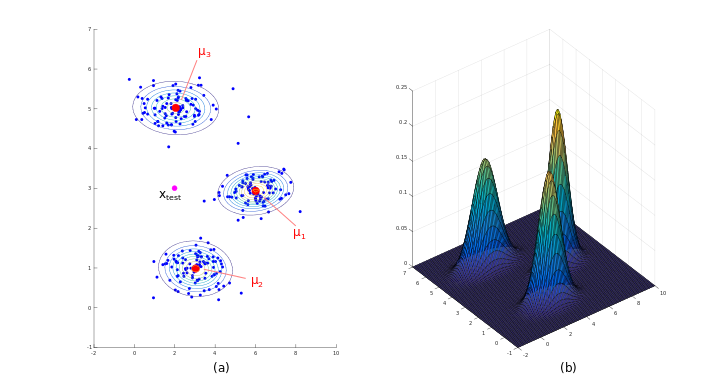
\includegraphics[width=\textwidth,height=3in]{gmmdemo.png}
\caption{Illustration of GMM on the 2d data set from Figure \ref{fig:kmeans-prog} with $K=3$. 
(a) Plot of the cluster means and variances indicated with ellipses. We have added a potention anomaly at $\bs x_{test}$. 
(b) Surface plot of the estimated density function $p(\bs x)$.}
\label{fig:gmm-demo}
\end{figure*}

A simple model selection tool is the ``elbow method''.
We have already discussed this method in section \ref{sect:kmeans-ms} in the context about $K$-means.
Instead of the distortion function, we plot the negative value of the log likelihood $-\ell(\bs\theta)$ at the optimum parameter value of $\bs\theta$ against $K$ and try to identify a ``kink".
Of course, this approach comes with the same drawbacks that were discussed earlier.

Alternatively, we can make use of statistical model selection tools.
A simple practical approach is to fit the GMM for a range of values of $K$ and evaluate the \emph{Bayesian Information Criterion} (BIC) for each of the models.
We then select the value of $K$ for which the BIC was lowest (see \cite{fraley2002} for more details).

In general, model selection for finite mixture models is a difficult problem and virtually all model selection tools have significant drawbacks. 
One way of circumventing the problem is to make the move to Bayesian non-parametric models that allow for automatic inference of the number of clusters.
A popular approach to non-parametric clustering is to use the Dirichlet process mixture model.

For more information on model selection in mixture models, see \cite{Murphy}.

\subsection{Implementation Details and Demonstration}

Beside the $K$-means algorithm, we have also implemented the Gaussian mixture model in C++ (using Armadillo \cite{armadillo}).
Again, implementing of the pseudo-code from Algorithm \ref{alg:gmm} is relatively straight-forward.
The only additions that we made are
\begin{enumerate}
\item We added an upper limit to the number of iterations of the EM algorihtm.
\item We used a mixed error test as convergence criterion.
This means that we stop the algorithm if
\begin{equation}
|\ell(\bs\theta^{\,(new)}) - \ell(\bs\theta^{\,(current)})| < \epsilon \left(1 + |\ell(\bs\theta^{\,(current)})|\right)
\end{equation}
where $\epsilon > 0$ is the target error.
\item Similar to $K$-means, we perform multiple runs of the EM algorithm with different random initializations to mitigate the risk of getting a poor local solution.
\end{enumerate}

Figure \ref{fig:gmm-demo} illustrates the use of GMM.
We applied the model to the same data set as in Figure \ref{fig:kmeans-prog} with $K=3$.
The resulting clusters are shown in panel (a), where we used ellipses to indicate the covariance parameters.
Panel (b) shows a surface plot of the estimated density function $p(\bs x)$.

We also show how the Gaussian mixture model can be applied to \emph{anomaly detection}.
In panel (a), we have included a potential anomaly at the point marked as $\bs x_{test}$.
Once we have an estimate for $p(\bs x)$, we can evaluate it at $\bs x_{test}$.
We flag $\bs x_{test}$ as an anomaly if 
\begin{equation*}
p(\bs x_{test}) < \epsilon
\end{equation*}
where $\epsilon > 0$ as a preset threshold.



\section{Conclusion and Further Work}
\label{sect:concl}
The EM algorithm is one of the most important techniques in machine learning and statistics.
As such, many extensions and variations of it have been proposed in the literature.
\cite{Murphy} gives a short description of several extensions of EM, while \cite{mclachlan1997} offers a more in-depth treatment.

An important extension is \emph{online EM}.
We discussed the EM algorithm in the context of \emph{batch learning}. 
However, when dealing with large data sets, this can be very slow, since the algorithm needs to go through the entire data set in order to produce a single parameter update.
The main alternative to batch learning is \emph{online learning}. 
In online learning algorithms, each iteration considers only a single data point in order to update the parameters.
In practice, this can lead to significant speedups.

There are two main variants of an online version of the EM algorithm.
They are known as \emph{incremental EM} and \emph{stepwise EM} and are discussed in \cite{liang2009}.

We showed how the EM algorithm can be used to fit latent variable models.
In particular, we derived the EM algorithm for the Gaussian mixture model and $K$-means.

Both, $K$-means and Gaussian mixtures play an important role in unsupervised machine learning.
They offer simple and intuitive approaches to clustering and are straightforward to implement.
Typically, they are included in any major machine learning software package.
In practice, this makes them a good ``first thing to try" in a wide range of clustering problems.

There a various ways in which the two models can be extended and generalized.
For instance, the \emph{elliptical $K$-means} algorithm \cite{sung1998} offers a hard-assignment version of the GMM with general covariance matrices.

Other extensions to the GMM seek to find better ways of infering the parameters of the model, for instance through Markov Chain Monte Carlo methods.

However, as we said before, the biggest limitations of finite mixture models is that we need to manually set the number of components $K$.
Model selection methods are fraught with difficulties and so it may be beneficial to use Bayesian nonparametric approaches to clustering that automatically infer the number of clusters.
The most widely used of these methods is the Dirichlet process mixture model. 
For more information, see \cite{Murphy, Teh2010a}.

%% The Appendices part is started with the command \appendix;
%% appendix sections are then done as normal sections
\appendix


%% References
%%
%% Following citation commands can be used in the body text:
%% Usage of \cite is as follows:
%%   \cite{key}         ==>>  [#]
%%   \cite[chap. 2]{key} ==>> [#, chap. 2]
%%

%% References with bibTeX database:
\section*{Bibliography}
\bibliographystyle{elsarticle-num}
\bibliography{references.bib}

%% Authors are advised to submit their bibtex database files. They are
%% requested to list a bibtex style file in the manuscript if they do
%% not want to use elsarticle-num.bst.

%% References without bibTeX database:

% \begin{thebibliography}{00}

%% \bibitem must have the following form:
%%   \bibitem{key}...
%%

% \bibitem{}

% \end{thebibliography}


\end{document}

%%
%% End of file `mini.tex'.